\problem{}
Consider a restaurant with $m$ different menu items. Each customer to the restaurant want to order one item, and each of them has a set of items they are willing to order from. The restaurant makes $d_i$ amount of item $i$, for $1 \leq i \leq m$, so that at most $d_i$ customers can order item $i$. Given $n$ customers, where the $j$'th customer has a list $C_j$ of items they are willing to order, design an efficient algorithm to maximize the number of customers you can serve.

\solution{}
\begin{figure}[htbp]
    \centering
    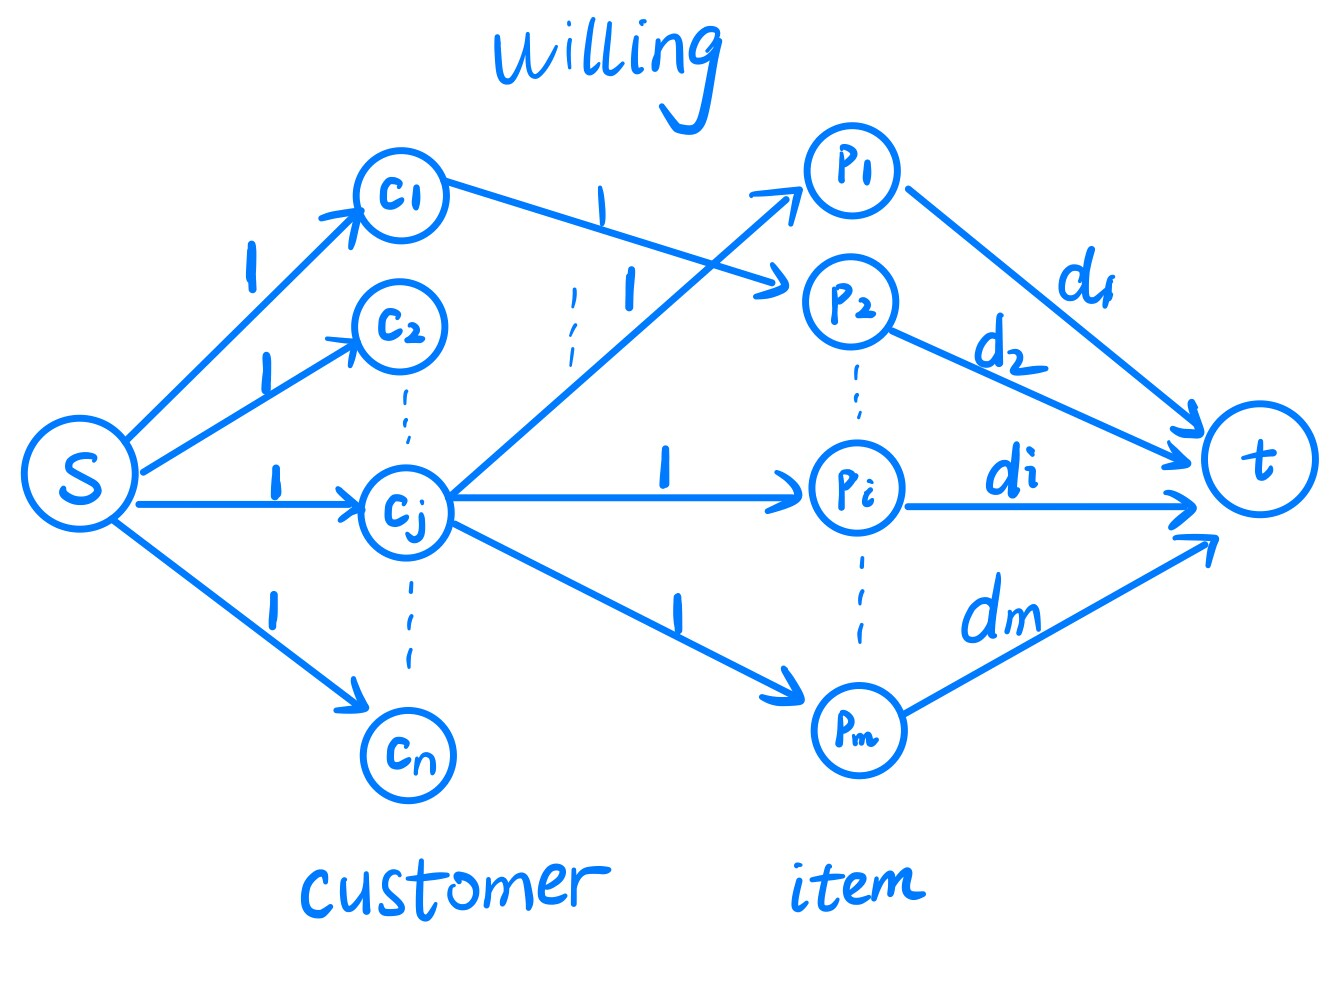
\includegraphics[width=\linewidth]{../fig/p3.png}
    \caption{Way to contrust the graph}
    \label{fig:p3}
\end{figure}
We can construct the graph as the Figure \ref{fig:p3} shows.

The details are as follows:\\
Let node $c_j$ represents the $j$-th customer, node $p_i$ represents the $i$-th item.\\
And $s$ to be the source node, $t$ to be the sink node.\\

Sice each customer will be satisfied if them get one item they want, so we can set up an edge from $s$ to each of the customer $c_j$ with capacity $1$.

Since the $j$-th customer has a list $C_j$ of items they are willing to order, so we can set up an edge from $c_j$ to each of the item $p_j\in C_j$ with capacity $1$.

Since the $i$-th item has been made in the number of $d_i$, so we can set up an edge from $d_i$ to $t$ with capacity $d_i$.

We can use the Ford-Fulkerson algorithm to find the maximum flow of the constructed graph.\\

The maximum number that the customers we can serve is the maximum flow on the constructed graph.\\
The time complexity is $O((nC+m)^2\log D)$,\\
where $C=\max\limits_{j=1,2,\cdots,n}\{|C_j|\},D=\max\limits_{i=1,2,\cdots,m}\{d_i\}$\\

\newpage